\documentclass{article}
\usepackage{color}
\usepackage[usenames,dvipsnames]{xcolor}
\usepackage{tikz}
\usepackage{textcomp}
\usepackage[top=1cm, bottom=1cm, left=1cm, right=1cm]{geometry}
\begin{document}
\definecolor{mygreen}{rgb}{0.57,0.64,0.27} 
\definecolor{mylightgreen}{rgb}{0.79,0.84,0.65} % light washed green
\pagecolor{mygreen}

\begin{center}
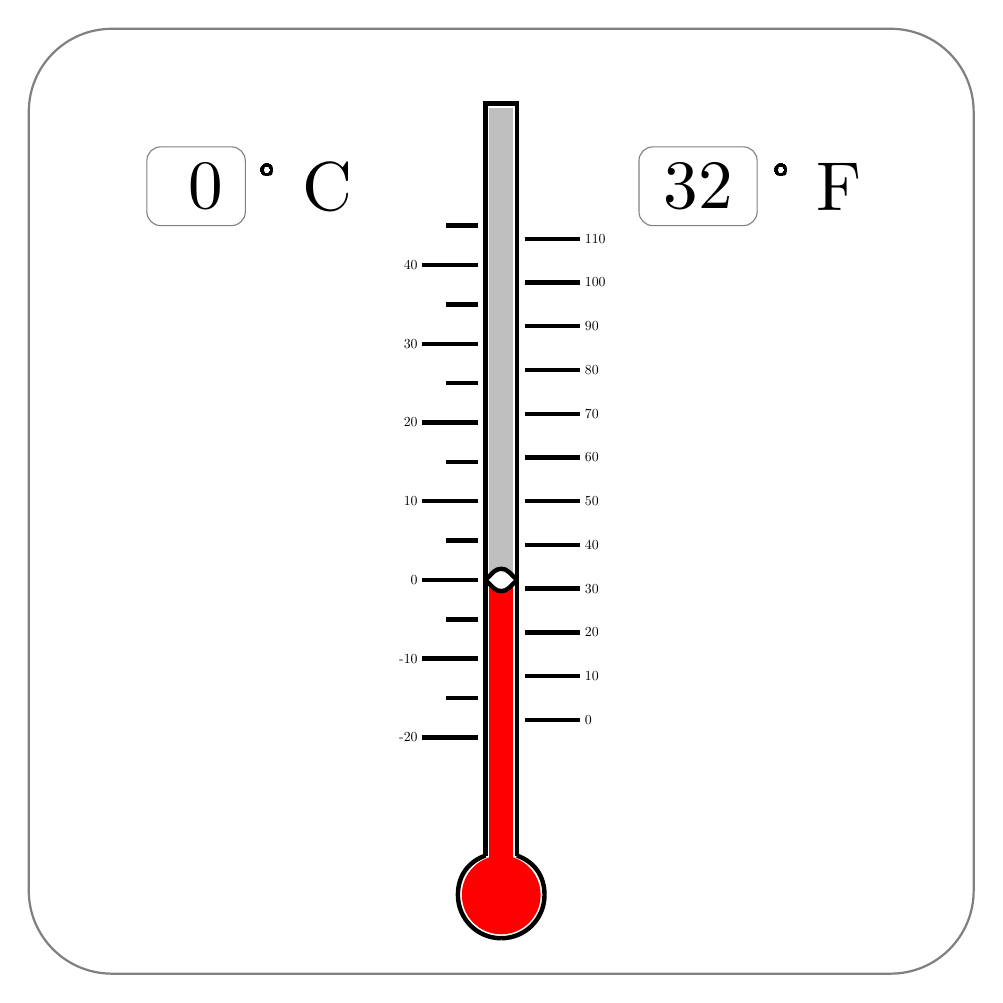
\begin{tikzpicture} [scale=0.5, transform shape]

% the border 
\draw [gray, thick=90, fill = white, rounded corners=30] (-12, -10) rectangle (12, 14);

% the red liquid
\path [fill=red] (0,-8) circle [radius=1];
\path [fill=red] (-0.3,-8) rectangle (0.3,0);
\path [fill=gray!50!] (-0.3, 0) rectangle (0.3, 12);
% the black boarder
\draw [black, ultra thick] (-0.4, -7) -- (-0.4, 12.1) -- (0.4, 12.1) -- (0.4, -7);
\draw [black, ultra thick] (0, -9.1) to [out=180, in=270] (-1.1, -8) to [out=90, in=200] (-0.4,-7);
\draw [black, ultra thick] (0, -9.1) to [out=0, in=270] (1.1, -8) to [out=90, in=340] (0.4,-7);

% Celsius meters
\draw [black, ultra thick] (-2, -4) -- (-0.6, -4);
\node [left] at (-2,-4) {-20};
\draw [black, ultra thick] (-1.4, -3) -- (-0.6, -3);
\draw [black, ultra thick] (-2, -2) -- (-0.6, -2);
\node [left] at (-2,-2) {-10};
\draw [black, ultra thick] (-1.4, -1) -- (-0.6, -1);
\draw [black, ultra thick] (-2, 0) -- (-0.6, 0);
\node [left] at (-2,0) {0};
\draw [black, ultra thick] (-1.4, 1) -- (-0.6, 1);
\draw [black, ultra thick] (-2, 2) -- (-0.6, 2);
\node [left] at (-2,2) {10};
\draw [black, ultra thick] (-1.4, 3) -- (-0.6, 3);
\draw [black, ultra thick] (-2, 4) -- (-0.6, 4);
\node [left] at (-2,4) {20};
\draw [black, ultra thick] (-1.4, 5) -- (-0.6, 5);
\draw [black, ultra thick] (-2, 6) -- (-0.6, 6);
\node [left] at (-2,6) {30};
\draw [black, ultra thick] (-1.4, 7) -- (-0.6, 7);
\draw [black, ultra thick] (-2, 8) -- (-0.6, 8);
\node [left] at (-2,8) {40};
\draw [black, ultra thick] (-1.4, 9) -- (-0.6, 9);

% Fahrenheit meters
\draw [black, ultra thick] (0.6, 8.666) -- (2, 8.666);
\node [right] at (2, 8.666) {110};
\draw [black, ultra thick] (0.6, 7.555) -- (2, 7.555);
\node [right] at (2, 7.555) {100};
\draw [black, ultra thick] (0.6, 6.444) -- (2, 6.444);
\node [right] at (2, 6.444) {90};
\draw [black, ultra thick] (0.6, 5.333) -- (2, 5.333);
\node [right] at (2, 5.333) {80};
\draw [black, ultra thick] (0.6, 4.222) -- (2, 4.222);
\node [right] at (2, 4.222) {70};
\draw [black, ultra thick] (0.6, 3.111) -- (2, 3.111);
\node [right] at (2, 3.111) {60};
\draw [black, ultra thick] (0.6, 2) -- (2, 2);
\node [right] at (2, 2) {50};
\draw [black, ultra thick] (0.6, 0.888) -- (2, 0.888);
\node [right] at (2, 0.888) {40};
\draw [black, ultra thick] (0.6, -0.222) -- (2, -0.222);
\node [right] at (2, -0.222) {30};
\draw [black, ultra thick] (0.6, -1.333) -- (2, -1.333);
\node [right] at (2, -1.333) {20};
\draw [black, ultra thick] (0.6, -2.444) -- (2, -2.444);
\node [right] at (2, -2.444) {10};
\draw [black, ultra thick] (0.6, -3.555) -- (2, -3.555);
\node [right] at (2, -3.555) {0};

% the readings
\begin{scope}[every node/.style={scale=5}]
% Celsius reading
\draw[gray, rounded corners=5] (-9,9) rectangle (-6.5,11);
\node[,color=black,,rounded corners=1] (Cbox) at (-7.5, 10) {0};
\node[,,color=black,,rounded corners=3] (CD) at (-5, 10) {\textdegree{} C};
% Fahrenheit reading
\draw[gray, rounded corners=5] (3.5,9) rectangle (6.5,11);
\node[,color=black,,rounded corners=1] (Fbox) at (5, 10) {32};
\node[,,color=black,,rounded corners=3] (FD) at (8, 10) {\textdegree{} F};
\end{scope}

% the handle
\draw [ultra thick, fill = white!20!, rounded corners] (-0.4, 0) -- (0, 0.4) -- (0.4, 0);
\draw [ultra thick, fill = white!20!, rounded corners] (-0.4, 0) -- (0, -0.4) -- (0.4, 0);
%\draw [ultra thick] (0,0) circle [radius=0.4];


\end{tikzpicture}
\end{center}



\end{document}